\documentclass[12pt,a4paper,titlepage]{article}
\usepackage{License_style}
\usepackage{pdfpages}
\usepackage{eso-pic}

  
\begin{document}
\pagenumbering{gobble}


\numberwithin{lstlisting}{section}


% TITLE
\begin{titlepage}
\selectlanguage{romanian}

\newcommand{\HRule}{\rule{\linewidth}{0.5mm}} % Defines a new command for the horizontal lines, change thickness here

\center

Ministerul Educației al Republicii Moldova\\ % Name of your university/college
Universitatea Tehnică a Moldovei \\% Name of your university/college
Facultatea de Calculatoare, Informatică și Microelectronică\\
Filiera Anglofonă "Computer Science"\\


\vspace{6cm}




\begin{center}
\Large \textbf{Definirea și gestiunea indecșilor}\\
\vspace{0.6cm}
Lucrare de curs\\ Baze de date și cunoștințe
\end{center}
\vspace{6cm}


\hfill Efectuat de: \\ \hfill N.Maxian\\
\vspace{0.2cm}
\hfill Verificat de: \\ \hfill I.Cojanu\\
\vspace{0.2cm}


% If you don't want a supervisor, uncomment the two lines below and remove the section above
%\Large \emph{Author:}\\
%John \textsc{Smith}\\[3cm] % Your name

%----------------------------------------------------------------------------------------
%	DATE SECTION
%----------------------------------------------------------------------------------------
\vfill % Fill the rest of the page with whitespace
\begin{center}
Chișinău 2017
\end{center}


\end{titlepage}
\selectlanguage{english}


\cleardoublepage


\tableofcontents

\newpage

\pagenumbering{arabic}
\setcounter{page}{10}
\setcounter{secnumdepth}{4}

\addtocontents{toc}{\protect\thispagestyle{empty}} % no page number on the table of contents page
\cleardoublepage


%LISTA FIGURILOR. Este recomandabila daca in text ai peste cel putin 10-15 FIGURI
\listoffigures
\addcontentsline{toc}{section}{List of figures}
\clearpage

%LISTA TABELELOR. Este recomandabila daca in text ai peste cel putin 10-15 tabele
\listoftables
\addcontentsline{toc}{section}{List of tables}
\clearpage

\lstlistoflistings
\addcontentsline{toc}{section}{Listings}
\clearpage

%INTRODUCERE
%\setcounter{page}{17} 
\phantomsection
\addcontentsline{toc}{section}{Introduction}
\section*{Introduction}
\phantomsection

A database index is a data structure that improves the speed of data retrieval operations on a database table at the cost of additional writes and storage space to maintain the index data structure. Indexes are used to quickly locate data without having to search every row in a database table every time a database table is accessed. Indexes can be created using one or more columns of a database table, providing the basis for both rapid random lookups and efficient access of ordered records.

An index is a copy of selected columns of data from a table that can be searched very efficiently that also includes a low-level disk block address or direct link to the complete row of data it was copied from. Some databases extend the power of indexing by letting developers create indexes on functions or expressions. 

Indexes are used in every database where performance matters. Although it has big benefit of performance improvement, we also have some consequences like:
\begin{itemize}
	\item More memory is used
	\item Add/Update/Delete operations on indexed columns, invokes index rebuild and makes this operations to be slower.
\end{itemize}

\clearpage
\cleardoublepage

% CAPITOLUL 1
\section{Problem and domain analysis}
\phantomsection

\subsection{Indexes}

A database index is a data structure that improves the speed of data retrieval operations on a database table at the cost of additional writes and storage space to maintain the index data structure. Indexes are used to quickly locate data without having to search every row in a database table every time a database table is accessed. Indexes can be created using one or more columns of a database table, providing the basis for both rapid random lookups and efficient access of ordered records.

An index is a copy of selected columns of data from a table that can be searched very efficiently that also includes a low-level disk block address or direct link to the complete row of data it was copied from. Some databases extend the power of indexing by letting developers create indexes on functions or expressions. 

\subsection{Indexes Usage}
\subsubsection{Support for fast lookup}
Most database software includes indexing technology that enables sub-linear time lookup to improve performance, as linear search is inefficient for large databases.

Suppose a database contains N data items and one must be retrieved based on the value of one of the fields. A simple implementation retrieves and examines each item according to the test. If there is only one matching item, this can stop when it finds that single item, but if there are multiple matches, it must test everything. This means that the number of operations in the worst case is O(N) or linear time. Since databases may contain many objects, and since lookup is a common operation, it is often desirable to improve performance.

An index is any data structure that improves the performance of lookup. There are many different data structures used for this purpose. There are complex design trade-offs involving lookup performance, index size, and index update performance. Many index designs exhibit logarithmic (O(log(N))) lookup performance and in some applications it is possible to achieve flat (O(1)) performance.

\subsubsection{Policing the database constraints}
Indexes are used to police database constraints, such as UNIQUE, EXCLUSION, PRIMARY KEY and FOREIGN KEY. An index may be declared as UNIQUE, which creates an implicit constraint on the underlying table. Database systems usually implicitly create an index on a set of columns declared PRIMARY KEY, and some are capable of using an already existing index to police this constraint. Many database systems require that both referencing and referenced sets of columns in a FOREIGN KEY constraint are indexed, thus improving performance of inserts, updates and deletes to the tables participating in the constraint.

Some database systems support an EXCLUSION constraint that ensures that, for a newly inserted or updated record, a certain predicate holds for no other record. This can be used to implement a UNIQUE constraint (with equality predicate) or more complex constraints, like ensuring that no overlapping time ranges or no intersecting geometry objects would be stored in the table. An index supporting fast searching for records satisfying the predicate is required to police such a constraint.

\subsection{Index architecture/Indexing Methods}

\subsubsection{Clustered}
Clustering alters the data block into a certain distinct order to match the index, resulting in the row data being stored in order. Therefore, only one clustered index can be created on a given database table. Clustered indices can greatly increase overall speed of retrieval, but usually only where the data is accessed sequentially in the same or reverse order of the clustered index, or when a range of items is selected.

Since the physical records are in this sort order on disk, the next row item in the sequence is immediately before or after the last one, and so fewer data block reads are required. The primary feature of a clustered index is therefore the ordering of the physical data rows in accordance with the index blocks that point to them. Some databases separate the data and index blocks into separate files, others put two completely different data blocks within the same physical file(s).

\subsubsection{Non-clustered}
The data is present in arbitrary order, but the logical ordering is specified by the index. The data rows may be spread throughout the table regardless of the value of the indexed column or expression. The non-clustered index tree contains the index keys in sorted order, with the leaf level of the index containing the pointer to the record (page and the row number in the data page in page-organized engines; row offset in file-organized engines).

In a non-clustered index,

The physical order of the rows is not the same as the index order.
The indexed columns are typically non-primary key columns used in JOIN, WHERE, and ORDER BY clauses.
There can be more than one non-clustered index on a database table.

\subsection{MSSQL Execution Plan}
A query plan, execution plan, or query execution plan is an algorithm showing a set of steps in a specific order that is executed to access data in a database

A query plan shows how a query was executed, or how it will be executed which is significant for troubleshooting query performance issues. Executing a SELECT statement to find out its query plan and effect on SQL Server performance can be acceptable, but executing UPDATEs to find that out is not an option. The plan is calculated by a SQL Server component Query Optimizer using minimum of server resources. When creating the SQL Server query execution plan, the number of database objects involved, joins, indexes and their availability, number of output columns, and more is considered

When a new query is executed, Query Optimizer evaluates the query plan, optimizes and compiles it, and stores it in the plan cache. The plan cache is a part of SQL Server buffer where data and query plans are stored (buffered), so they can be reused later

When a query is executed, Query Optimizer first searches the plan cache looking for a query plan that can be reused, thus making the execution faster. If there’s no query plan that can be reused, a new one has to be created, which takes time and therefore makes query execution last longer

A very useful characteristic of query plans is that when a stored procedure is executed, the query plan is created for the stored procedure name and the same query plan will be reused whenever the stored procedure is executed, despite the values specified for procedure parameters. When it comes to executing ad hoc queries, query plans are created based on complete code, so different parameters or any change in code will prevent reuse of the existing plan. This clearly indicates what should be done to make your code run faster – wrap it up as stored procedures or functions, and the existing query plans will be reused and therefore code will be executed much faster

The slow execution of ad hoc queries can be mitigated by using the Optimize for ad hoc workloads option, introduced in SQL Server 2008. The option optimizes the plan cache use, as it solves the situation when query plans executed only once fill up the plan cache. As the buffer cache is used for both data and plan buffering, and the percentage of cache used for each changes in time depending on the current situation, it’s necessary to use the cache wisely. Instead of buffering the whole plan, when the option is set to “True”, only a fragment of the plan is buffered when the query is executed for the first time. When an ad hoc query is executed for the second time, its complete plan is buffered in the cache


\subsection{MSSQL Execution Plan Elements}
Since we are using Indexes for optimization of database, we need to know great tools given by Microsoft like Execution Plan. Execution Plan tells us what happens behind of query, what operations are done,what cost has every operations and how are merged together. We will use this functionality for analyzing effects of Indexation. 
\\
Although execution plan has a lot of elements, in this course work we will cover only few definitions such as Scan,Seek and types of Joins. 

\subsubsection{Scan}
Since a scan touches every row in the table, whether or not it qualifies, the cost is proportional to the total number of rows in the table. Thus, a scan is an efficient strategy if the table is small or if most of the rows qualify for the predicate.
\begin{figure}[ht!]
	\centering
	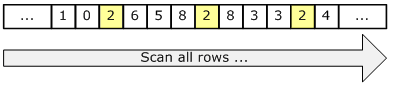
\includegraphics[width=0.6\textwidth]{scan}
	\caption{Scan algorithm}
\end{figure}

\subsubsection{Seek}
Since a seek only touches rows that qualify and pages that contain these qualifying rows, the cost is proportional to the number of qualifying rows and pages rather than to the total number of rows in the table.

Index Scan is nothing but scanning on the data pages from the first page to the last page. If there is an index on a table, and if the query is touching a larger amount of data, which means the query is retrieving more than 50 percent or 90 percent of the data, and then the optimizer would just scan all the data pages to retrieve the data rows. If there is no index, then you might see a Table Scan (Index Scan) in the execution plan.

Index seeks are generally preferred for the highly selective queries. What that means is that the query is just requesting a fewer number of rows or just retrieving the other 10 (some documents says 15 percent) of the rows of the table.
\begin{figure}[ht!]
	\centering
	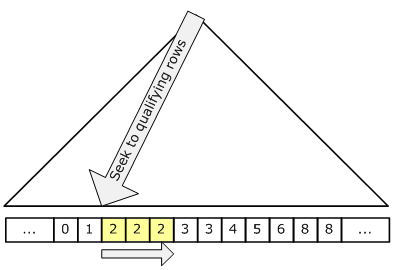
\includegraphics[width=0.6\textwidth]{seek}
	\caption{Seek algorithm}
\end{figure}

\subsubsection{SQL Joins \cite{SQLJoins}}
SQL Server employs three types of join operations:

\begin{itemize}	
	\item Nested loops joins
	\item Merge joins
	\item Hash joins
\end{itemize}

If one join input is small (fewer than 10 rows) and the other join input is fairly large and indexed on its join columns, an index nested loops join is the fastest join operation because they require the least I/O and the fewest comparisons. For more information about nested loops, see Understanding Nested Loops Joins.

If the two join inputs are not small but are sorted on their join column (for example, if they were obtained by scanning sorted indexes), a merge join is the fastest join operation. If both join inputs are large and the two inputs are of similar sizes, a merge join with prior sorting and a hash join offer similar performance. However, hash join operations are often much faster if the two input sizes differ significantly from each other. For more information, see Understanding Merge Joins.

Hash joins can efficiently process large, unsorted, non indexed inputs.
\\
For examples we can look into \cite{Joins}.

\subsection{Problem definition}
Main scope of this course work is to demonstrate indexation and it's benefits.So we will divide our problem into two parts.
\begin{itemize}
	\item Clustered Index
	\item Non Clustered Index
\end{itemize}
Both subproblems will have their own purpose and own examples. Each subproblem has an definition,analysis,solution and post-analysis. 

\clearpage
\cleardoublepage
%
%CAPITOLUL2
\section{MSSQL implementation. Particularities}
\subsection{Preparing database}
\subsubsection{Downloading database}
In this Course Work I will use database Adventure Works \cite{AdventureWorks}. 
\begin{figure}[ht!]
	\centering
	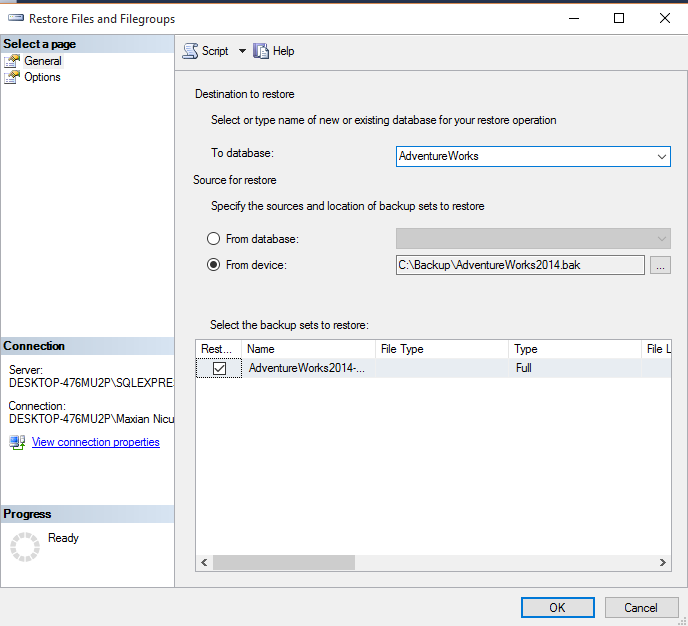
\includegraphics[width=0.8\textwidth]{restore}
	\caption{Restoring AdventureWorks database}
\end{figure}

\subsubsection{Droping database indexes}
In order to show why we should use indexes, let remove all indexes for following tables:
\begin{itemize}
	\item Production.Product
	\item Production.ProductCategory
	\item Person.EmailAddress
	\item Person.Password
	\item Person.Person
	\item Person.PersonPhone\textsl{}
	\item Person.PhoneNumberType
\end{itemize}

\subsection{Clustered Indexes}
\subsubsection{Problem definition}
Let's assume we have following query, which extracts ProductId, Name,Category and StandartCost from database.
\lstinputlisting[style=mystyle, language=SQL, caption={Finding product with a given id}]{sourcecode/productSearch.sql}

\subsubsection{Analysis of execution plan}
\begin{figure}[ht!]
	\centering
	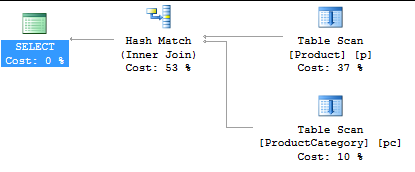
\includegraphics[width=0.5\textwidth]{product_find}
	\caption{Execution plan for the query}
\end{figure}

From this execution plan, we see that our query has cost of \textbf{0.034}. Furthermore, since our tables have no clustered indexes, data is stored as a heap, in the file. We see that our algorithm scans table for finding needed row. This means that query takes row by row and tries to find needed row that matches our criterions. This is ok for few rows, but when we have thousands of rows, performance will hurt us. 

\subsubsection{Solution}
Of course Clustered Indexes. Clustered Indexes rearranges our table data as a b-tree structure. Let's create clustered index on Product table, with column ProductId. Now we can find needed product at once, without scanning all entire data ! Once we found product, we have also ProductSubCategoryId, which is also an clustered index for ProductCategory table, so we access that table also by id.


\lstinputlisting[style=mystyle, language=SQL, caption={Creating clustered indexes}]{sourcecode/productIndexes.sql}

\subsubsection{Final results}

\begin{figure}[ht!]
	\centering
	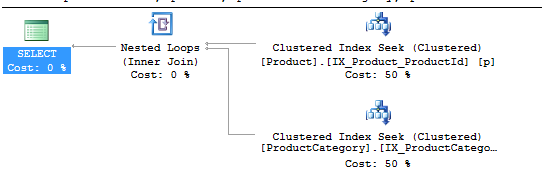
\includegraphics[width=0.6\textwidth]{product_after_indexes}
	\caption{Execution plan after creating clustered indexes}
\end{figure}

Now we can see that we have \textbf{Clustered Index Seek}. This is faster way to find a data. This means we have no more loops, scan and everything that costs us data. Having ProductID, we can directly access Address of data, where row is situated. So, we have optimized our query as much as possible ! Now we have total cost of \textbf{0.0065}, 80\% less than initial. That is awesome !



\subsection{Non Clustered Indexes}
\subsubsection{Problem definition}
Here we will try to extract basic data such as FirstName,LastName,Email,Password,PasswordHash,Phone,PhoneType for each Person based on following tables:
\begin{itemize}
	\item EmailAddress
	\item Password
	\item Person
	\item PersonPhone
	\item PhoneNumberType
\end{itemize}
\lstinputlisting[style=mystyle, language=SQL, caption={Selecting person base information}]{sourcecode/personInfo.sql}

\subsubsection{Analysis of execution plan}
\begin{figure}[ht!]
	\centering
	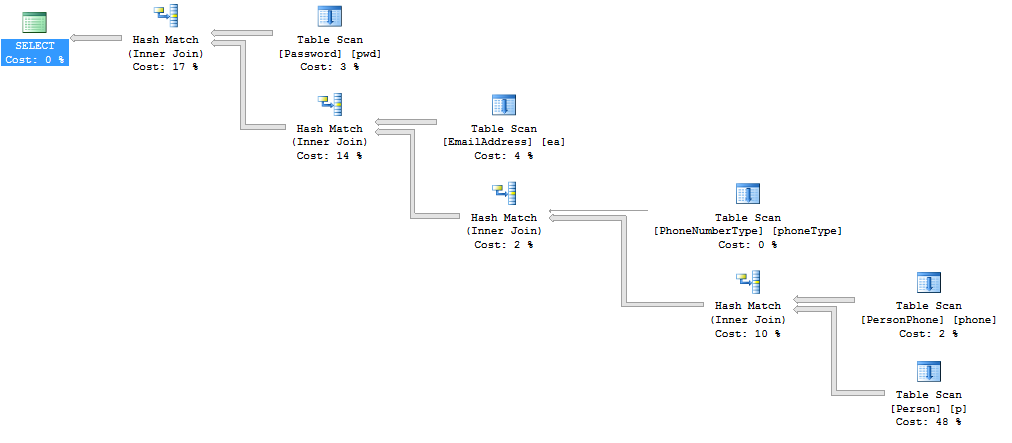
\includegraphics[width=1\textwidth]{person_analysis}
	\caption{Execution plan for the query}
\end{figure}

Hence, we obtained an cost of \textbf{5.94} for our query with 19972 rows.

Since we don't have any index here, we can observe that in execution plan we have only "Table scan". This means in our query, SQL engine scan table row by row, which is very slow. 

\subsubsection{Solution}
In order to optimize it, let's to improve our queries with Non Clustered indexes. This means that, instead of big tables we will search into smaller index tables, which contains less data and can be found with a given index.

Since we have 13 columns on \textbf{Person} table, it make us to have a big overhead when extracting data. Since we assume we will execute a lot of times this query, we need to optimize this. Non-clustered indexes are great for this. We could "shrink" our data table by creating smaller index table. We will create index on \textbf{BussinessEntittyID} column because we use this column in JOIN clauses. We also need \textbf{FirstName} and \textbf{LastName} information from that table, we also define this columns to be included into non-clustered index table. Same things we will do for each table, in order to optimize our query and remove overhead which we acutally don't need.

\lstinputlisting[style=mystyle, language=SQL, caption={Creating non-clustered indexes}]{sourcecode/personNonClusteredIndex.sql}

\subsubsection{Final results}
\begin{figure}[ht!]
	\centering
	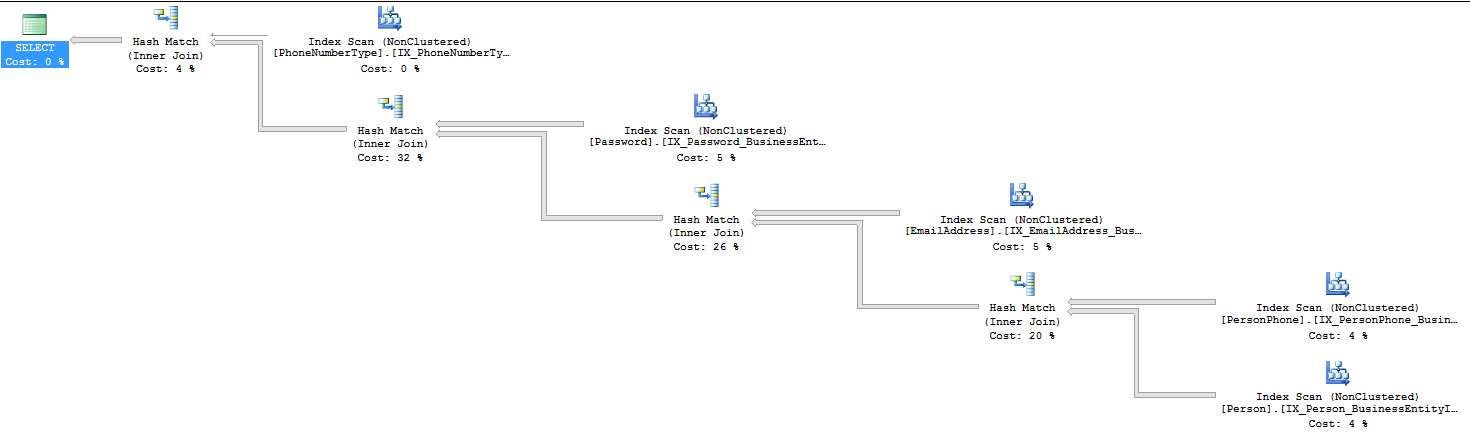
\includegraphics[width=1\textwidth]{person_analysis_after}
	\caption{Execution plan after non-clustered index creation}
\end{figure}

Now, we see that instead of table scan we have Index Scan. Which is faster than what we had. Also now we have in indexes everything what we need, so no need to lookup into the table for missing columns.

Now we have an cost of \textbf{3.12}, which is 48\% less than we had before. Nice ! It's an improvement.

\clearpage
\cleardoublepage

%CAPITOLUL3
\section{Practical part}
\phantomsection

\subsection{Differences and Similarities between MSSQL and Oracle}
Since MSSQL was base SQL Database for my course work, here I will define things that are different in SQL Database.

\subsubsection{Execution plan}
In SQL Developer to show execution plan, you should press F10 or click the Explain Plan icon. Of course it looks different and has it's features which makes him different of what we have in SSMS.

\begin{figure}[ht!]
	\centering
	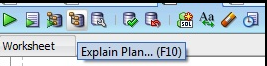
\includegraphics[width=0.4\textwidth]{sqldeveloper_execution_plan}
	\caption{Showing execution plan}
\end{figure}

\subsubsection{Changes index creation queries}
Because Oracle SQL doesn't have \textbf{INCLUDE} statement on creating indexes. To migrate our queries we need only to change queries which have \textbf{INCLUDE} statement.

\lstinputlisting[style=mystyle, language=SQL, caption={Finding product with a given id}]{sourcecode/migration.sql}

\clearpage
\cleardoublepage


% IMPORTANT REMARK  
% If your table of contents need to be splitted in two parts (in order to accomodate the frame used for TOC)
% within the body text, right before the chapter/section that you want to be started on anew page, 
% you should add:     \addtocontents{toc}{\protect\newpage}

%CONCLUZII
\phantomsection
\addcontentsline{toc}{section}{Conclusions}
\section*{Conclusions}
\phantomsection

From my point of view, Indexation should be know by everyone who is planning and developing a database. Indexes gives us a better performance for our database and queries which are important for you, and needs to be optimized. By defining indexes, we are creating new index table which has references to original data table, or could include data directly in it, as we have done in our case. Of course, we cannot make everything an index ! After changing table data or changed columns, SQL will perform an index rebuild ! We need to know that rebuild = time. So, we need to make sure that we have enough indexes to make database faster and not many to make it work slower due the indexes rebuild. Indexes are key factor for performance, once you have a good database architecture. 


Also I would say that MSSQL Execution Plan is a very very useful feature for SSMS. It shows us every steps what SQL is doing in order to give you an result. Execution Plan gives you imagination on what happens behind the query. Using this tool we can optimize our queries and indexes. 

\clearpage
\cleardoublepage

\cleardoublepage
\addcontentsline{toc}{section}{References}
\begin{thebibliography}{99999}
\phantomsection
\singlespace\normalsize

\bibitem{AdventureWorks} Adventure Works 2014 - Full database \url{https://msftdbprodsamples.codeplex.com/downloads/get/880661}


\bibitem{SQLJoins} Advanced Query Tuning Concepts \url{http://msdn.microsoft.com/en-us/library/ms191426\%28v=SQL.100\%29.aspx}

\bibitem{IndexSeekScan} Index Seek vs Index Scan
\url{https://blog.sqlauthority.com/2007/03/30/sql-server-index-seek-vs-index-scan-table-scan/}

\bibitem{Joins} LOOP, HASH and MERGE Join Types
\url{http://www.madeiradata.com/loop-hash-and-merge-join-types/}

\end{thebibliography}

\cleardoublepage
   
 
\end{document}